\chapter{A Precise Half-Wave Rectifier}


\section{Objectives}
\begin{itemize}
    \item To verify two precise half-wave rectifiers
\end{itemize}

\section{Materials}
\begin{itemize}
    \item Breadboard
    \item DC power supply
    \item Digital Multi-Meter
    \item \hyperref[1N4148]{Diode (1N4148)}
    \item Function Generator
    \item \hyperref[LM741_1]{Op.Amp. (LM741)}
    \item Oscilloscope
    \item Resistors
\end{itemize}

\section{Introduction}
    \subsection{Circuit Diagram}
    \begin{figure}[h]
    \centering
    \begin{subfigure}[h]{0.45\textwidth}
        \centering
        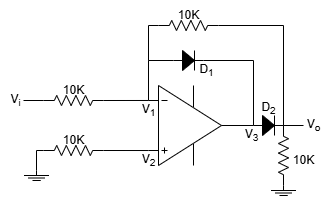
\includegraphics[width=0.7\linewidth]{Lab12/Lab12a.drawio.png}
        \caption{}
        \label{lab12a}
        \end{subfigure}
    \hfill
        \begin{subfigure}[h]{0.45\textwidth}
        \centering
        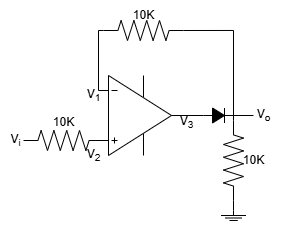
\includegraphics[width=0.7\linewidth]{Lab12/Lab12b.drawio.png}
        \caption{}
        \label{lab12b}
        \end{subfigure}
    \caption{Two precise half-wave rectifiers}
    \label{lab12f}
    \end{figure}
    \FloatBarrier

\section{Detailed Procedures}
    \subsection{Analyzation}
    \begin{itemize}
        \item In the Fig.\ref{lab12a}, Condition for Not-Saturation is $V_I>V_\gamma-V^+$.\\
            When $V_I>0$, $D_1$ on, $D_2$ off:\\
            \begin{equation}
                \begin{cases}
                    V_o = 0\\
                    V_3 = V_1 - V_\gamma = V_2 - V_\gamma\\
                \end{cases}
            \end{equation}
            When $V_I<0$, $D_1$ off, $D_2$ on:\\
            \begin{equation}
                \begin{cases}
                    V_o = -V_I\\
                    V_3 = V^+ + V_\gamma\\
                \end{cases}
            \end{equation}
        \item In the Fig.\ref{lab12b}, Condition for Not-Saturation is $0<V_I<V^+-V_\gamma$.\\
            When $V_I<0$, $D$ off, no negative feedback:\\
                \begin{equation}
                    \begin{cases}
                        V_3 = V^-\\
                        V_o = 0\\
                    \end{cases}
                \end{equation}
            When $V_I>0$, $D$ on, negative feedback (virtual short):\\
                \begin{equation}
                    \begin{cases}
                        V_o = V_I\\
                        V_3 = V_o + V_\gamma = V_I+ V_\gamma ~(<V^+)\\
                    \end{cases}
                \end{equation}
    \end{itemize}
        Overall, from the equations above we can obtain:\\
            \begin{itemize}
                \item In Fig.\ref{lab12a},
                    \begin{equation*}
                    V_o =
                        \begin{cases}
                            0 & V_I>0\\
                            -V_I & V_I<0\\
                        \end{cases}
                    \end{equation*}
                \item In Fig.\ref{lab12b},
                    \begin{equation*}
                    V_o =
                        \begin{cases}
                            V_I & V_I>0\\
                            0 & V_I<0\\
                        \end{cases}
                    \end{equation*}
            \end{itemize}

    \subsection{Procedures}
    Construct the circuit as Fig.\ref{lab12f} with supply voltages at $\pm$12V*.\\
    {\small *Requirement for $\pm$10V but we used $\pm$12V instead.}\\
        \begin{itemize}
            \item \textbf{AC}
                \begin{itemize}
                    \item For Fig.\ref{lab12a},\\
                    \item For Fig.\ref{lab12b},\\
                \end{itemize}

            \item \textbf{DC}
                \begin{itemize}
                    \item For Fig.\ref{lab12a},\\
                        \begin{table}[h]
                        \centering
                        \begin{tabular}{|c|c|c|c|c|c|c|}
                            \hline
                            vi & -10   & -5    & -1      & 1      & 5      & 10     \\ \hline
                            v1 & -0.05 & 0     & -0.0015 & -0.003 & -0.05  & -0.05  \\ \hline
                            v2 & 0     & 0     & 0       & 0      & 0      & 0      \\ \hline
                            v3 & 10.5  & 5.583 & 1.518   & -0.5   & -0.58  & -0.62  \\ \hline
                            vo & 9.857 & 4.973 & 0.991   & -0.001 & -0.001 & -0.002 \\ \hline
                        \end{tabular}
                        \end{table}
                        \FloatBarrier
                    \item For Fig.\ref{lab12b},\\
                        \begin{table}[h]
                        \centering
                        \begin{tabular}{|c|c|c|c|c|c|c|c|c|}
                            \hline
                            vi & -12     & -10    & -5     & -1     & 1     & 5     & 10     & 12     \\ \hline
                            v1 & -0.001  & 0      & 0      & 0      & 0.995 & 5     & 9.937  & 11.925 \\ \hline
                            v2 & -11.969 & -9.99  & -4.996 & -0.995 & 0.996 & 4.99  & 9.995  & 10.582 \\ \hline
                            v3 & -9.98   & -11.99 & -11.99 & -11.99 & 1.49  & 5.576 & 10.557 & 11.202 \\ \hline
                            vo & 0       & 0      & 0      & 0      & 0.996 & 5     & 9.948  & 10.59  \\ \hline
                        \end{tabular}
                        \end{table}
                        \FloatBarrier
                \end{itemize}
            
        \end{itemize}
\section{Discussion}
    The results are very closed to theoretical values might because we used the DC voltage of $\pm$12.

\section{Conclusion}